\chapter{\IfLanguageName{dutch}{Tunnel technologieën}{Tunneling methods}}%
\label{ch:tunnel-technologieën}

Voor de opzet van een tunnel tussen twee toestellen zijn verschillende methoden mogelijk. Allereerst zijn er de verschillende netwerkmodellen (lagen) waarop een tunnel kan worden opgezet:
\begin{itemize}
    \item \textbf{Layer 2-tunneling:} Deze methode simuleert een directe verbinding op datalinkniveau, alsof de twee verbonden apparaten zich in hetzelfde lokale netwerk (LAN) bevinden. Dit kan handig zijn bij toepassingen die afhankelijk zijn van broadcastverkeer of MAC-adressen. Voorbeelden van Layer 2-tunneling zijn Ethernet over GRE, L2TP en VXLAN.
    \item \textbf{Layer 3-tunneling:} Hierbij wordt er op netwerkniveau (IP-laag) een verbinding opgezet tussen twee netwerken of toestellen. Alle data tussen de twee punten wordt geëncrypteerd verzonden. Typische voorbeelden zijn IPsec, OpenVPN en WireGuard.
\end{itemize}
Binnen de huidige opstelling is gekozen voor L2TP als Layer 2-tunneltechnologie, omdat deze eenvoudig te configureren is (en later te automatiseren) en compatibel is met de systemen die in deze opstelling worden gebruikt.
Voor de Layer 3-tunnel is gekozen voor OpenVPN, om verschillende redenen: het is open-source, waardoor de configuratie kan worden afgestemd op de vereisten van dit project; 
het kan draaien op bijna elke poort, wat het mogelijk maakt om firewalls te omzeilen (zoals in deze opstelling het geval is); 
en het werkt goed samen met L2TP, zonder de complexiteit die gepaard gaat met het configureren van IPsec.

\section{L2TP}
\label{sec:layer2}


\subsection{Structuur}

Een L2TP-tunnel bestaat uit een gemeenschappelijk headerformaat dat controle- en databerichten onderscheidt. Belangrijke velden in de header zijn o.a. het \textit{Type}-bit (controle of data), Tunnel ID, Session ID, en sequentienummers voor betrouwbaarheid bij controleberichten. 
Controleberichten (zoals \texttt{SCCRQ}, \texttt{SCCRP}, \texttt{SCCCN}) regelen het opzetten, beheren en afbreken van tunnels en sessies. Authenticatie gebeurt meestal via een CHAP-uitwisseling tijdens de tunnelopbouw. Databerichten encapsuleren PPP-frames en worden niet opnieuw verzonden bij verlies.
\\

Een tunnel wordt opgezet tussen een L2TP Access Concentrator (LAC) en een L2TP Network Server (LNS). Verkeer over de tunnel wordt verstuurd via UDP (meestal poort 1701), wat efficiënte transmissie mogelijk maakt en problemen met TCP-over-TCP voorkomt.
Tot slot maakt L2TP gebruik van een hiërarchie waarbij meerdere sessies binnen één tunnel mogelijk zijn. Data wordt driemaal encapsuleerd: eerst met een L2TP-header, daarna met een UDP-header, en tot slot met een IP-header. Fragmentatie gebeurt alleen op IP-niveau, niet binnen L2TP zelf.

\begin{figure}[H]
    \centering
    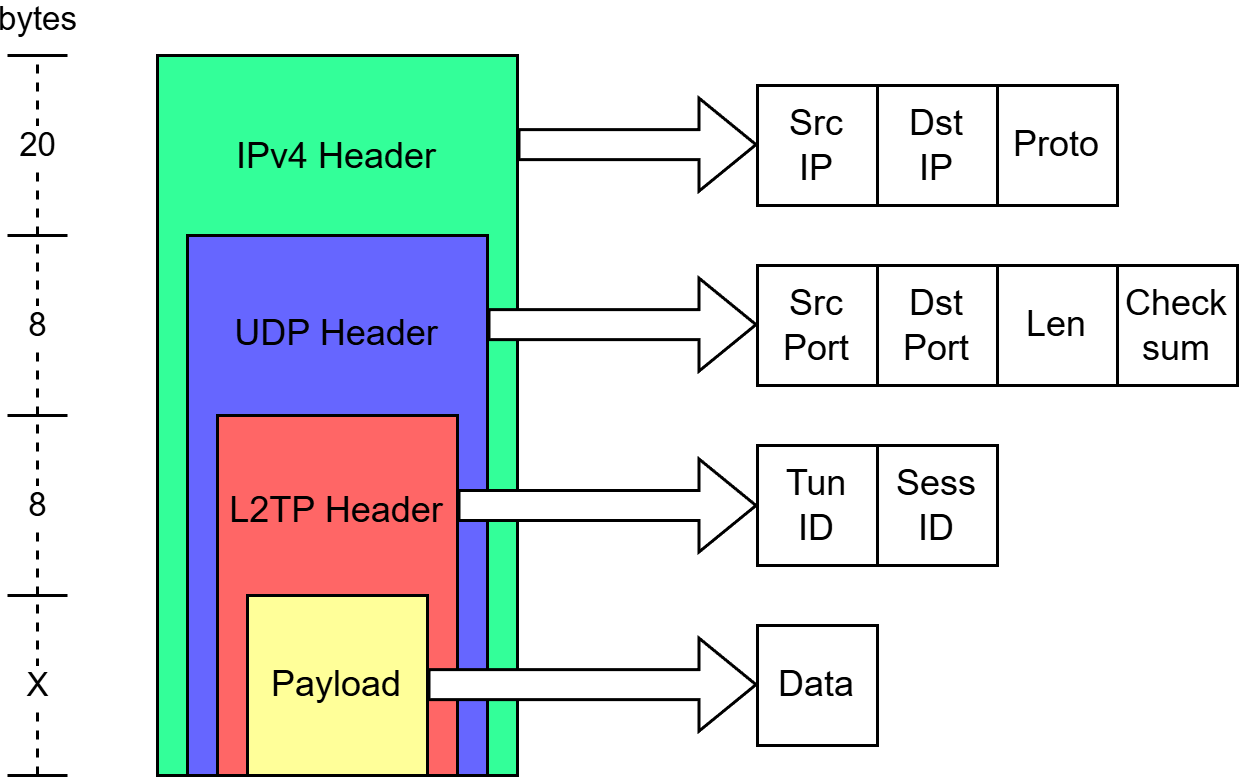
\includegraphics[width=1\textwidth]{PacketStructureL2TP.png}
    \caption[Structuur van L2TP]{\label{fig:L2TPStructure}Een simpele visualisatie van de structuur van een L2TP packet.}
\end{figure}

\subsection{Configuratie}
Voor het opzetten van een verbinding tussen twee IP-adressen via L2TP is geen extra software nodig, aangezien dit kan worden uitgevoerd met de ingebouwde functies van het IP-protocol en het besturingssysteem zelf.
Dit is ook zichtbaar in de code die hieronder wordt weergegeven.
\begin{listing}[H]
\begin{minted}{bash}
    sudo ip l2tp add tunnel tunnel_id 1000 peer_tunnel_id 2000 encap udp local 192.168.1.2 remote 10.0.0.2 udp_sport 1701 udp_dport 2000
    sudo ip l2tp add session tunnel_id 1000 session_id 1000 peer_session_id 2000
    sudo ip link set l2tpeth0 mtu 1400
    sudo ip link set dev l2tpeth0 up
    sudo brctl addif s6 l2tpeth0
\end{minted}
\caption[Configuratie L2TP Server]{De gebruikte shell-commando's om een L2TP tunnel op te zetten op de server (IDLab).}
\end{listing}

De getoonde commando's gebruiken het `ip`-hulpmiddel om een L2TPv3-tunnel op te zetten tussen twee hosts over UDP. 
Eerst wordt een tunnel gedefinieerd met lokale en externe IP-adressen en UDP-poorten (voor de opstelling zijn dit dan publieke IP addressen). 
Vervolgens wordt een sessie aangemaakt binnen die tunnel. Daarna wordt het virtuele netwerkapparaat (`l2tpeth0`) geconfigureerd en geactiveerd. 
Ten slotte wordt dit apparaat toegevoegd aan een bestaande bridge (`s6`), zodat het deel uitmaakt van het virtuele Layer 2-netwerk.


\subsection{Performantie}

Van de drie mogelijkheden is deze theoretisch gezien de snelste, aangezien L2TP de minste overhead genereert.
Bij een minimale configuratie bedraagt de header van een L2TP-pakket ongeveer 8~bytes.

Tijdens de configuratie en opzet van de tunnel werd een MTU-waarde van 1400~bytes ingesteld, om te garanderen dat er geen fragmentatie optreedt bij het verzenden van data.
Deze waarde zorgt ervoor dat de effectieve gegevensinhoud van een enkel pakket nooit groter is dan 1400~bytes. Hierdoor blijft er ongeveer 100~bytes beschikbaar voor de resterende overhead van L2TP-, IP- en UDP-headers.
Dit is gebaseerd op de standaard MTU-waarde van 1500~bytes die in de meeste netwerken wordt gehanteerd.
\\

Bij het testen op de toestellen werden volgende waarden vastgesteld voor de snelheid:

TODO

\section{OpenVPN tunnels}
\label{sec:openvpn}

\subsection{Structuur}

Een OpenVPN-tunnel bestaat uit twee soorten pakketten: controlepakketten, gebruikt voor TLS-handshakes en sessiebeheer, en datapakketten, die geëncrypteerd gebruikersverkeer vervoeren. Controlepakketten bevatten informatie zoals sessie-ID’s, sleutel-ID’s en HMAC’s. Datapakketten bevatten een initialisatievector (IV), geëncrypteerde payload en optioneel een compressievlag.
Het opzetten van een tunnel verloopt via een TLS-handshake waarbij certificaten worden uitgewisseld en tijdelijke sleutels worden gegenereerd met Elliptic Curve Diffie-Hellman.
OpenVPN maakt gebruik van moderne encryptiestandaarden zoals AES-256-GCM en beschermt tegen replay-aanvallen via packet-ID-controle. In servermodus kunnen duizenden clients tegelijkertijd worden beheerd via sessie-multiplexing met unieke peer-ID’s.

\begin{figure}[H]
    \centering
    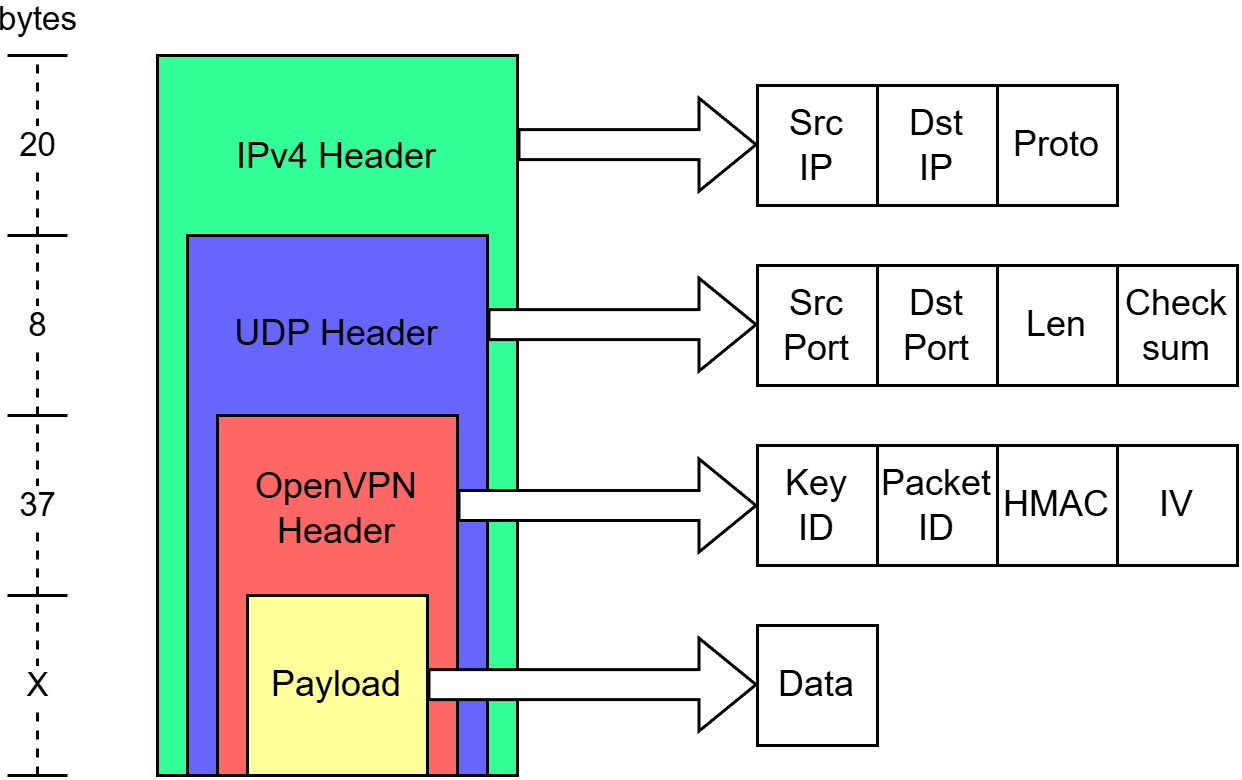
\includegraphics[width=1\textwidth]{PacketStructureOpenVPN.png}
    \caption[Structuur van OpenVPN]{\label{fig:OpenVPNStructure}Een simpele visualisatie van de structuur van een OpenVPN packet.}
\end{figure}

\subsection{Configuratie}

Voor de opstelling van OpenVPN wordt gebruikgemaakt van een client-serverarchitectuur, waarbij de OpenVPN-server zich bevindt op de node in het IDLab en de client een server is die zich in het klaslokaal bevindt.
De configuratie en opzet van een OpenVPN-verbinding is uitgebreider dan die van een L2TP-tunnel en verloopt in meerdere fasen.
\\

De eerste stap bestaat uit het aanmaken van certificaten en sleutels via EasyRSA. Hierbij wordt eerst een Public Key Infrastructure (PKI) opgezet, vervolgens wordt een Certificate Authority (CA) aangemaakt. 
Daarna genereert men een certificaataanvraag (CSR), die vervolgens ondertekend wordt met de CA. 
Ook wordt er een Diffie-Hellman-sleutel op basis van elliptische krommen (Elliptic Curve Diffie-Hellman) gegenereerd.
Deze procedure wordt vervolgens herhaald voor de client die verbinding zal maken met de server.
Daarna genereert men een ta.key (TLS-authenticatiebestand) en wordt de OpenVPN-server opgestart.

\begin{listing}[H]
\begin{minted}{bash}
    sudo apt update && sudo apt upgrade -y
    sudo apt install openvpn easy-rsa -y

    make-cadir /etc/easyrsa-setup
    cd /etc/easyrsa-setup

    ./easyrsa init-pki
    ./easyrsa build-ca

    ./easyrsa gen-req server nopass
    ./easyrsa sign-req server server
    ./easyrsa gen-dh

    cd /etc/openvpn
    openvpn --genkey --secret /etc/openvpn/ta.key
    nohup openvpn --verb 3 --config server.conf
\end{minted}
\caption[Configuratie OpenVPN Server]{De gebruikte shell-commando's om een OpenVPN tunnel op te zetten op de server (IDLab).}
\end{listing}

Vanwege beperkingen binnen het IDLab wordt de server niet via systemd gestart, maar met behulp van \texttt{nohup}, zodat deze blijft draaien op de achtergrond zonder aan een actieve terminal gekoppeld te zijn.
Het is belangrijk dat bij het opstarten van de OpenVPN-server de juiste paden naar de benodigde bestanden (zoals certificaten en sleutels) correct zijn opgenomen in het configuratiebestand. 
Een fout hierin kan ertoe leiden dat de server niet succesvol opstart.

\begin{listing}[H]
\begin{minted}{bash}
    port 1194
    proto udp
    dev tun
    ca /etc/easyrsa-setup/pki/ca.crt
    cert /etc/easyrsa-setup/pki/issued/server.crt
    key /etc/easyrsa-setup/pki/private/server.key
    dh /etc/easyrsa-setup/pki/dh.pem
    tls-auth ta.key 0
    cipher AES-256-CBC
    user nobody
    group nogroup
    persist-key
    persist-tun
    status openvpn-status.log
    log-append  /var/log/openvpn.log
    verb 3
\end{minted}
\caption[Configuratie bestand OpenVPN Server]{De structuur van het configuratiebestand van OpenVPN op de server (IDLab).}
\end{listing}

De laatste stap bestaat uit het overzetten van de gegenereerde certificaten, sleutels en de ta.key van de server naar de client.
Deze bestanden zijn noodzakelijk om een beveiligde verbinding tot stand te brengen. Dit volgt het principe van een pre-shared key, 
waarbij zowel de server als de client over gedeelde vertrouwelijke gegevens beschikken om de verbinding te verifiëren en op te zetten.

\subsection{Performantie}

Op het vlak van performantie is deze manier van werken theoretisch trager, aangezien het gebruik van OpenVPN gepaard gaat met een grotere hoeveelheid overhead in vergelijking met een L2TP-verbinding.
Zelfs bij een minimale configuratie bedraagt de OpenVPN-header al 37~bytes, terwijl de header bij L2TP slechts 8~bytes bedraagt. 
Deze toename in overhead is het gevolg van de aanwezigheid van meerdere controle- en identificatievelden in het OpenVPN-pakket. 
Deze extra informatie is noodzakelijk om te garanderen dat de verzonden data enkel leesbaar is voor het bedoelde eindpunt, 
en draagt bij aan de beveiliging van de verbinding.
\\

Door de grotere overhead is de hoeveelheid effectieve data die per pakket kan worden verstuurd kleiner. 
Hierdoor zijn er meer pakketten nodig om dezelfde hoeveelheid data te verzenden, wat een impact kan hebben op het netwerkverkeer en de belasting op de toestellen die de VPN-verbinding verwerken.
\\

Hoewel dit dus zwaarder en theoretisch trager is, is het voordeel dat de data veilig is en niet zomaar kan worden uitgelezen door derden, wat bij L2TP mogelijk wel het geval is.
Bij het testen op de toestellen werden volgende waarden vastgesteld voor de snelheid:

TODO


\section{Combinatie van L2TP en OpenVPN}
\label{sec:combinatie}

\subsection{Hoe}

\subsection{Waarom}

\subsection{Performantie}